\documentclass{article}
\usepackage{tikz}
\usetikzlibrary{backgrounds}
\begin{document}
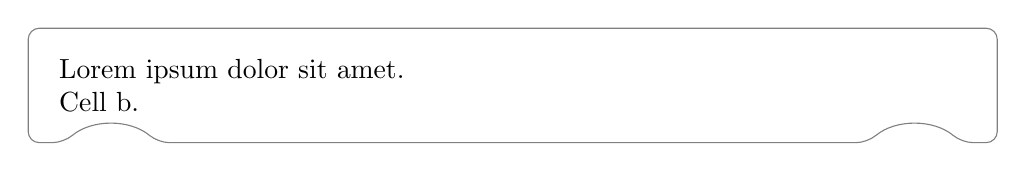
\begin{tikzpicture}
  \node[text width=.95\linewidth, inner sep=11pt] (m) {Lorem ipsum dolor sit amet.\\ Cell b.};
  \pgfonlayer{background}
  \draw[rounded corners,gray,fill=white] (m.north west) -- (m.north east) -- (m.south east) -- ++(-.45cm,0) to[bend right=40] ++(-1.2cm,0) -- ([xshift=1.65cm]m.south west) to[bend right=40] ++(-1.2cm,0) -- ++(-.45cm,0) -- cycle;
  \endpgfonlayer
\end{tikzpicture}
\gdef\SatexReachedEnd{}
\end{document}
